\documentclass[12pt,a4paper,openright,twoside]{book}
\usepackage[utf8]{inputenc}
\usepackage{disi-thesis}
\usepackage{code-lstlistings}
\usepackage{notes}
\usepackage{shortcuts}
\usepackage{acronym}

\school{\unibo}
\programme{Corso di Laurea in Ingegneria e Scienze Informatiche}
\title{B-Tree File System per piattaforme IoT}
\author{Leonardo Marcaccio}
\date{\today}
\subject{Ricerca Operativa}

\supervisor{Marco Antonio Boschetti}

\session{III}
\academicyear{2023-2024}

\mainlinespacing{1.241}

\begin{document}

\frontmatter\frontispiece

\begin{abstract}
    Questa Tesi esplora il processo di studio, progettazione e implementazione di un prototipo di \textit{File System} basato sulla struttura dati \textit{B-Tree}, sviluppato per la piattaforma \textit{Internet of Things} (\textit{IoT}) IOtto di Onit S.p.A.

    L'obiettivo principale è migliorare l'efficienza nella gestione e nel recupero dei dati, affrontando le problematiche tipiche di un \textit{File System} come la scalabilità e l'ottimizzazione delle risorse.

    Il lavoro comprende un'analisi dello stato dell'arte sui moderni \textit{File System}, con particolare attenzione alla loro interazione con i sistemi \textit{IoT}. Viene approfondito il principio di funzionamento del \textit{B-Tree}, dimostrando come questa struttura dati possa essere sfruttata per realizzare una struttura performante e affidabile.

    Inoltre, vengono descritte le fasi di progettazione e implementazione, evidenziando le soluzioni adottate per adattare il prototipo alle esigenze specifiche della piattaforma IOtto.

    I risultati preliminari mostrano che il prototipo proposto garantisce significativi miglioramenti in termini di velocità di accesso ai dati e utilizzo delle risorse rispetto alle alternative tradizionali.
\end{abstract}

\begin{dedication}
    Alla mia famiglia, per il loro costante supporto e incoraggiamento.
\end{dedication}

%----------------------------------------------------------------------------------------
\tableofcontents
\listoffigures
\lstlistoflistings
%----------------------------------------------------------------------------------------

\mainmatter

%----------------------------------------------------------------------------------------
\chapter{Introduzione}
\label{chap:Introduzione}
%----------------------------------------------------------------------------------------

    \section{Struttura della Tesi}

        Questa Tesi è articolata in quattro capitoli principali.

        \begin{itemize}
            \item Questo primo capitolo introduce il problema affrontato, delineando il contesto di riferimento e gli obiettivi del lavoro.
            \item Il secondo capitolo fornisce le basi teoriche del lavoro, offrendo una panoramica sui moderni \textit{File System} e sulla loro connessione con il mondo dell’\textit{IoT}. Viene inoltre approfondita la struttura dati \textit{B-Tree}, evidenziandone le proprietà principali e la sua rilevanza rispetto al problema affrontato.
            \item Il terzo capitolo si concentra sulla progettazione e sull’implementazione del prototipo di \textit{File System}. Vengono descritte le scelte effettuate durante il processo di sviluppo e spiegato come il \textit{B-Tree} sia stato utilizzato per soddisfare le esigenze specifiche della piattaforma IOtto.
            \item Infine, il quarto capitolo discute i risultati ottenuti dalla valutazione del prototipo. Vengono inoltre presentate le conclusioni tratte dallo studio e delineate le possibili direzioni per future modifiche e sviluppi relativi al prodotto.
        \end{itemize}

    \section{Premesse e Contesto}
    \label{sec:Premesse e Contesto}

        \subsection{Onit}

            Onit S.p.A. è un’azienda italiana all’avanguardia nel settore delle soluzioni IT e della consulenza, dedicata al miglioramento del management e dell’organizzazione aziendale.

            L'azienda offre un portafoglio diversificato di soluzioni software che spaziano da \textit{Operations \& Supply Chain} a \textit{Healthcare}, \textit{Business Analytics}, \textit{Web \& Mobile} e \textit{ICT System Integration}.

            Si caratterizza per la sua capacità di integrare sistemi eterogenei e di supportare la trasformazione digitale nelle imprese, promuovendo innovazione, efficienza operativa e competitività nel mercato moderno.

        \subsection{IOtto}

            \textit{IOtto} rappresenta la soluzione \textit{IoT} sviluppata da Onit per favorire la connettività tra macchinari, servizi e persone, realizzando così l’ideale di Industria 4.0.

            La piattaforma offre un controllo completo e in tempo reale degli impianti e dei macchinari, grazie a una serie di funzionalità integrate, tra cui:
            \begin{itemize}
                \item \textbf{IOtto Platform}: consente il monitoraggio e il controllo centralizzato degli impianti, supportando una completa digitalizzazione delle attività produttive.
                \item \textbf{IOtto Edge}: permette l’elaborazione e l’analisi dei dati direttamente “al margine” della rete, riducendo la latenza e ottimizzando il traffico informativo.
                \item \textbf{Asset Management System (AMS)}: facilita la gestione strategica della manutenzione, anticipando possibili anomalie e riducendo i tempi di intervento.
            \end{itemize}.

            Questa soluzione consente di ottimizzare i processi produttivi, ridurre i costi operativi, offrendo alle aziende il controllo totale sui propri impianti e una gestione predittiva degli asset.

    \section{Descrizione del problema}

        L'attuale \textit{File System} utilizzato dall'applicativo risulta non essere più ottimale nel contesto attuale, data la crescita e la mole dei dati gestiti.
        Risulta dunque necessario trovare un'alternativa che soddisfi le necessità attuali e future, in ambito di scalabilità e ottimizzazione.

    \section{Obiettivo di Tesi}

        L'obiettivo della Tesi risulta essere quello di realizzare un prototipo di \textit{File System} che sia scalabile, in grado di effettuare rapide letture e scritture, strutturalmente solido e ottimizzato nell'allocazione di spazio.

        In particolare, il lavoro si concentra sulla progettazione e realizzazione di un prototipo alternativo al sistema preesistente, con l'intento non solo di mantenere le prestazioni attuali, ma, ove possibile, di migliorarle.

        \subsection{Domande}
        \label{subsec:Domande}

            Segue ora un elenco di domande che sono state poste durante le prime fasi del progetto, al fine di identificare le esigenze e le aspettative del cliente.

            \begin{itemize}
                \item Quali tipi di dati devono essere memorizzati e gestiti?
                \item Qual è la quantità stimata di dati da gestire a regime?
                \item Quali saranno le dimensioni massime dei file e la granularità delle operazioni sui dati?
                \item Come garantire un basso consumo di risorse?
                \item Qual è la struttura di archiviazione più adatta?
                \item Il File System dovrà scalare per gestire un numero crescente di dispositivi IoT?
                \item Qual è la strategia per l'espansione dello spazio di archiviazione?
                \item Come gestire guasti hardware o interruzioni improvvise di alimentazione?
                \item È necessario prevedere meccanismi di backup o snapshot per i dati?
                \item Come si possono introdurre nuove funzionalità senza compromettere i dati esistenti?
            \end{itemize}

        \subsection{Scopo}

            L’obiettivo finale è quello di apportare un significativo miglioramento al software esistente, sfruttando l’hardware già disponibile per ottenere prestazioni più elevate.

            Questo intervento mira a incrementare le capacità del prodotto, garantendo una maggiore efficienza e un’esperienza d’uso più soddisfacente per i clienti.

            In particolare, il miglioramento si traduce nell’ottimizzazione delle funzionalità attuali e nell’ampliamento delle possibilità offerte dal sistema, lavorando direttamente sul software.

            Questo approccio consente di massimizzare il valore del prodotto, andando incontro alle crescenti aspettative degli utenti e mantenendo un vantaggio competitivo sul mercato.

\chapter{Stato dell'Arte}

    \section{L'Internet of Things}

        Il concetto di \textit{Internet of Things}, o in italiano \textit{Internet delle Cose}, rappresenta un'evoluzione nell'utilizzo della rete Internet, in cui gli oggetti, o ``cose", diventano riconoscibili e acquisiscono la capacità di comunicare dati attraverso la rete e di accedere a informazioni aggregate da altre fonti.

        Uno dei primi utilizzi di questo termine risale al 2001, in un documento del centro Auto-ID\footnote{Auto-ID Labs è un gruppo di ricerca nel campo dell'identificazione a radiofrequenza (RFID) in rete.
        } relativo alla creazione del network EPC\footnote{EPC, acronimo di Electronic Product Code, è uno standard identificativo universale che fornisce un'identità ad ogni oggetto fisico in qualsiasi parte del mondo.}.

        Tuttavia, non esiste un'origine univoca o un creatore effettivo del termine, poiché il concetto si è sviluppato progressivamente attraverso contributi di diversi ricercatori e innovatori nell'arco di tempo che va dai primi anni '90 fino al 2010.

        Gli oggetti connessi, che costituiscono il cuore pulsante dell’\textit{IoT}, sono definiti ``\textit{Oggetti Intelligenti}" (\textit{Smart Objects}) e si caratterizzano per proprietà distintive come la capacità di identificarsi, connettersi, localizzarsi, elaborare dati e interagire con l'ambiente circostante.

        Attraverso tecnologie come le \textit{Etichette RFID} (Identificatori a Radiofrequenza) o i \textit{Codici QR}, questi oggetti e luoghi possono comunicare informazioni tramite la rete o dispositivi mobili.

        L'obiettivo principale dell’\textit{IoT} risulta essere dunque il tentativo di creare una mappatura elettronica del mondo fisico, attribuendo un’identità digitale agli oggetti e ai luoghi che lo compongono.

        Sono nate inoltre organizzazioni come EPCglobal \footnote{ organizzazione globale per la gestione dello standard EPC} e Open Geospatial Consortium (o OGC)\footnote{organizzazione internazionale no-profit, che si occupa di definire specifiche tecniche per i servizi geospaziali e di localizzazione.} che lavorano per creare standard globali per la visibilità dei dati e l’utilizzo di sensori connessi via Web.

        In conclusione, le applicazioni dell’\textit{IoT} sono molteplici e variano dai processi industriali alla logistica, dalla logistica all’efficienza energetica, fino all’assistenza remota e alla salvaguardia ambientale.

        \cite{uckelmann2011architecting}\cite{hersent2011internet}\cite{chaouchi2013internet}

    \section{File System}

        I software, durante la loro esecuzione, si trovano di fronte alla sfida di dover gestire una grande quantità di informazioni. Per questo motivo, hanno bisogno di un sistema per archiviare temporaneamente i dati necessari al loro funzionamento. Una possibile soluzione è quella di utilizzare lo spazio di indirizzamento, un'area di memoria dedicata a questo scopo.

        \pagebreak

        Questo metodo di gestione dei dati però non è privo di problematiche:

        \begin{itemize}
            \item Capacità limitata, in quanto lo spazio di indirizzamento virtuale limita la quantità di dati archiviabili, rendendolo inadeguato per applicazioni che richiedono un'ampia archiviazione di dati, come sistemi bancari o database.
            \item Le informazioni memorizzate nello spazio di indirizzamento di un processo sono altamente volatili e vengono perse al termine del processo stesso.
            \item Non è permesso l'accesso concorrente. Spesso è necessario che più processi possano accedere contemporaneamente alle stesse informazioni, ma il confinamento dei dati all'interno di un unico processo lo impedisce.
        \end{itemize}

        Per rispondere a queste sfide, l'archiviazione a lungo termine richiede il rispetto di tre requisiti fondamentali:

        \begin{itemize}
            \item La possibilità di memorizzare grandi quantità di informazioni.
            \item La persistenza delle informazioni, anche dopo la terminazione del processo.
            \item L'accesso simultaneo ai dati da parte di più processi.
        \end{itemize}

        Per affrontare queste problematiche, è stato sviluppato il concetto di \textit{File System}, una componente fondamentale dei sistemi informatici progettata per permettere la gestione completa dei dati, inclusa la loro creazione, modifica, archiviazione e recupero all'interno di un sistema.

        Un \textit{File System}, al suo livello più alto, fornisce dunque un modo organizzato per archiviare, recuperare e gestire informazioni su supporti di archiviazione permanenti come i dischi.

        Esistono diversi approcci alla gestione dell'archiviazione permanente, poiché il problema è ampio e offre numerose soluzioni possibili.

        \cite{giampaolo1998practical}\cite{tanenbaum2015modern}

    \section{Categorizzazione dei File System}

        I \textit{File System} possono essere suddivisi in diverse categorie in base a specifiche caratteristiche, tra cui il livello di organizzazione gerarchica.

        Di seguito, analizziamo due tipologie principali di \textit{File System} in relazione alla loro struttura gerarchica.


        \subsection{Single-Level Directory Systems}

            Questo tipo di \textit{File System} rappresenta la forma più basilare e semplice di organizzazione dei dati. Consiste in una singola \textit{Directory}, spesso denominata \texttt{root}, che contiene tutti i file del sistema.

            Non esistono ulteriori livelli o \textit{Sottodirectory}: tutti i file sono archiviati in un unico spazio condiviso.

            \begin{figure} [h]
                \centering
                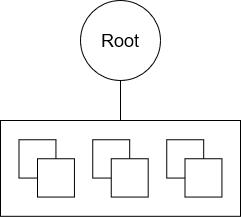
\includegraphics[width=.4\linewidth]{figures/SingleDirSystem.png}
                \caption{Esempio di Single Level Directory System}
                \label{fig:single-level-directory}
            \end{figure}

            L'approccio a livello unico offre alcuni vantaggi distinti. In primo luogo, la semplicità della struttura lo rende facile da implementare e utilizzare, poiché non sono necessari meccanismi complessi per navigare tra \textit{Directory} o \textit{Sottodirectory}.

            Inoltre, la localizzazione dei file è immediata, poiché tutto ciò che è presente all'interno del sistema è contenuto in una singola cartella, rendendo inutile un sistema di ricerca avanzato.

            Tuttavia, questo modello ha limitazioni significative, soprattutto per applicazioni più complesse o ambienti che richiedono la gestione di un elevato numero di file.

            Per questo motivo, i sistemi a directory singola sono utilizzati principalmente in dispositivi \textit{Embedded} o sistemi con esigenze limitate, come fotocamere digitali o dispositivi elettronici di consumo di base. In tali contesti, la semplicità e la leggerezza dell'architettura superano le necessità di una maggiore organizzazione.

        \subsection{Hierarchical Directory Systems}

            A differenza del modello a singolo livello, i sistemi a \textit{Directory Gerarchica} sono progettati per rispondere alle esigenze dei moderni ambienti informatici, caratterizzati dalla gestione di grandi volumi di dati e file.

            \begin{figure} [h]
                \centering
                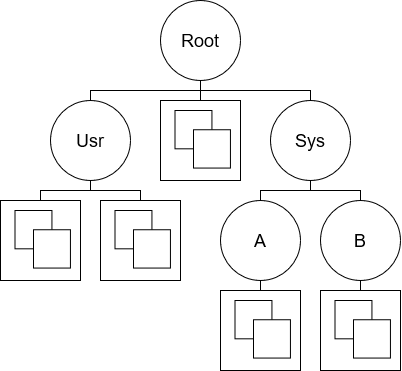
\includegraphics[width=.5\linewidth]{figures/MultipleDirSystem.png}
                \caption{Esempio di Hierarchical Directory System}
                \label{fig:hierarchical-directory}
            \end{figure}

            In questo tipo di \textit{File System}, è possibile creare una struttura organizzata composta da \textit{Directory} e \textit{Sottodirectory}. Questa struttura consente di suddividere i file in categorie o gruppi logici, favorendo una gestione più efficiente e un accesso più rapido alle informazioni.

            L'organizzazione gerarchica risulta particolarmente utile quando il sistema deve gestire elevate quantità di file. La possibilità di classificare i file in \textit{Directory} dedicate consente di mantenere ordine e chiarezza, riducendo la complessità che deriverebbe dall'avere tutto in un'unica directory.

            Un ulteriore vantaggio di questo approccio emerge nei contesti multiutente, dove più utenti condividono lo stesso \textit{File Server}. In questi casi, ogni utente può disporre di una \textit{Directory} \texttt{root} personale, che funge da punto di partenza per una gerarchia dedicata.

            Questa configurazione garantisce non solo la separazione dei dati tra gli utenti, ma anche un livello di personalizzazione che si adatta alle esigenze individuali.

    In conclusione, mentre i sistemi a livello singolo sono ideali per applicazioni semplici e specifiche, i sistemi gerarchici rappresentano una soluzione robusta e scalabile per ambienti complessi e moderni. \cite{tanenbaum2015modern}

    \section{Le Strutture Dati}

        Una \textit{Struttura Dati} è un modo per memorizzare e organizzare i dati al fine di facilitare l'accesso e le modifiche.

        Sono elementi fondamentali nella progettazione e nell'implementazione dei \textit{File System}, poiché determinano come i dati vengono organizzati, memorizzati e recuperati, influenzando direttamente l'efficienza e le prestazioni delle operazioni sui dati.

        Nessuna struttura dati singola è ottimale per tutti gli scopi, quindi è importante conoscere i punti di forza e le limitazioni delle diverse strutture.

        La scelta della struttura dati appropriata dipende da vari fattori, tra cui le esigenze specifiche del sistema, le prestazioni richieste e le limitazioni hardware.

        Tra le strutture dati più comuni utilizzate nei \textit{File System}, si possono citare:

        \begin{itemize}
            \item \textit{\textbf{Linked List}}: Una sequenza di nodi collegati tra loro, in cui ogni nodo contiene un riferimento al nodo successivo.
            \begin{figure} [h]
                \centering
                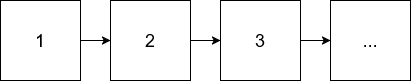
\includegraphics[width=.4\linewidth]{figures/LinkedList.png}
                \caption{Esempio di Linked List}
                \label{fig:linked-list}
            \end{figure}

            \item \textit{\textbf{Array}}: Una collezione di elementi disposti in una sequenza lineare, in cui ogni elemento è accessibile tramite un indice numerico.
            \begin{figure} [h]
                \centering
                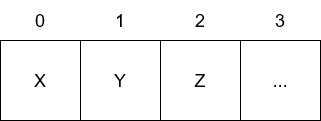
\includegraphics[width=.3\linewidth]{figures/Array.png}
                \caption{Esempio di Array}
                \label{fig:array}
            \end{figure}

            \item \textit{\textbf{Tree}}: Una struttura gerarchica composta da nodi collegati tra loro in maniera aciclica. In essa, ogni nodo (eccetto la radice) ha un solo nodo genitore e può generare uno o più nodi figli.
            \begin{figure} [h]
                \centering
                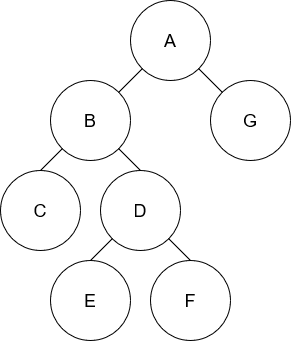
\includegraphics[width=.25\linewidth]{figures/Tree.png}
                \caption{Esempio di Tree}
                \label{fig:generic-tree}
            \end{figure}

            \item \textit{\textbf{Hash Table}}: Una struttura dati che associa chiavi a valori, consentendo un accesso rapido e diretto ai dati.
            \begin{figure} [h]
                \centering
                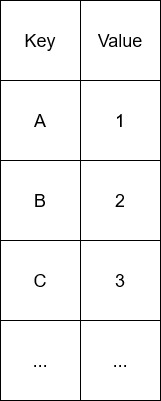
\includegraphics[width=.15\linewidth]{figures/HashTable.png}
I               \caption{Esempio di Hash Table}
                \label{fig:hash-table}
            \end{figure}
        \end{itemize}

        \cite{cormen2022introduction}

    \section{Strutture Dati Basate sui Tree}

        Le strutture dati come \textit{Linked List} e \textit{Array} sono strumenti potenti per rappresentare relazioni lineari, dove gli elementi sono disposti in una sequenza. Tuttavia, non tutte le relazioni nel mondo reale sono lineari.

        Molti problemi richiedono la rappresentazione di relazioni gerarchiche o ramificate, dove un elemento può essere connesso a più elementi in modo non sequenziale.

        Un \textit{Tree} è una struttura dati non lineare composta da nodi collegati tra loro in modo gerarchico. Ogni albero ha un \textit{Nodo Radice} denominato \texttt{Root} da cui partono uno o più \textit{Nodi} denominati \textit{Figli}, e ogni \textit{Figlio} può a sua volta avere altri \textit{Figli}, formando una struttura ramificata.

        In questo capitolo esploreremo le principali tipologie di alberi, le loro caratteristiche, i vantaggi e gli svantaggi.

        \subsection{Binary Trees}

            Un \textit{Binary Tree} è la variante più basilare dei \textit{Tree} in cui ogni nodo può avere al massimo due figli, chiamati \textit{Figlio Sinistro} e \textit{Figlio Destro}, ed è rappresentato tramite tre attributi per nodo: \texttt{Key} (Il Valore), \texttt{Left} (Figlio Sinistro) e \texttt{Right} (Figlio Destro).

            Questa struttura è semplice, versatile e ampiamente utilizzata per realizzare strutture dati più avanzate.

            Un \textit{Binary Tree} risulta essere semplice, efficiente e flessibile, ma può risultare inefficiente in caso di sbilanciamento e non è adatto a rappresentare relazioni con più di due figli.

        \subsection{Binary Search Trees}

            Un \textit{Binary Search Tree} (abbreviato \textit{BST}) è un tipo di \textit{Binary Tree} in cui ogni nodo rispetta un ordine: il valore del nodo è maggiore di tutti i valori nel suo sottoalbero sinistro e minore di tutti quelli nel sottoalbero destro.

            \pagebreak

            Questa struttura è utile per operazioni efficienti di ricerca, inserimento e cancellazione, e mantiene i nodi ordinati, semplificando operazioni come la ricerca del minimo o del massimo.

            Tuttavia, se l'albero non è bilanciato, può degenerare in una lista collegata perdendo così tutti i suoi benefici.

        \subsection{Balanced Trees}
            I \textit{Balanced Trees}, come \textit{AVL} e \textit{Red-Black}, sono \textit{Binary Search Trees} che mantengono l'altezza logaritmica rispetto al numero di nodi per garantire efficienza.

            Sia gli \textit{AVL} che i \textit{Red-Black Trees} utilizzano algoritmi e regole specifiche per mantenere l'equilibrio.

            Entrambi offrono prestazioni garantite come ricerca, inserimento e cancellazione in tempi brevi, rendendoli ideali per applicazioni che richiedono velocità e prevedibilità.

            Tuttavia, la gestione del bilanciamento richiede algoritmi più complessi rispetto ai \textit{BST} standard, con un maggiore overhead computazionale dovuto alle operazioni di bilanciamento.

        \subsection{N-ary Trees}

            Un \textit{n-ary Tree} è una generalizzazione dei \textit{Binary Trees} in cui ogni nodo può avere fino a \textit{n} figli, con \textit{n} come costante.

            Può essere rappresentato tramite \textit{Array} o \textit{Liste di Puntatori} ai figli ed è utile per relazioni con un numero fisso di figli, come negli alberi di decisione nei giochi di scacchi.

            Il problema principale con gli \textit{n-ary Tree} è la scelta del valore di \textit{n}.

            Se il valore è troppo piccolo, le operazioni risultano efficienti, ma può verificarsi uno spreco di memoria quando molti nodi hanno meno di \textit{n} figli, e la struttura risulta rigida per relazioni con un numero variabile di figli.

            Mentre se il valore è troppo grande, oltre a causare uno spreco di memoria, la struttura tende a diventare troppo simile ad una \textit{Linked List}, con un aumento della complessità computazionale.

        \cite{cormen2022introduction}

    \section{B-Tree}

        Un \textit{B-Tree} è un \textit{Balanced Search Tree} progettato per mantenere i dati ordinati e permettere operazioni di ricerca, inserimento e cancellazione in tempo logaritmico.

        A differenza di altri \textit{Balanced Trees} come i \textit{Red-Black Trees}, i \textit{B-Tree} sono ottimizzati per ridurre al minimo il numero di accessi al disco, rendendoli ideali per applicazioni che gestiscono grandi quantità di dati su dispositivi di memorizzazione secondaria.

        Indicando con \( n \) il numero massimo di nodi figli a cui un nodo può puntare, un \textit{B-Tree} ha le seguenti proprietà:

        \begin{itemize}
            \item Il numero massimo di \textit{Chiavi} per nodo è \( n - 1 \).
            \item Il \textit{Nodo Root} è un \textit{Nodo Foglia} o un \textit{Nodo Interno} con un numero di figli compreso tra \( 2 \) e \( n \) e un numero di chiavi compreso tra \( 1 \) e \( n - 1 \).
            \item Tutti gli altri \textit{Nodi Interni} hanno un numero di figli compreso tra \( n / 2 \) e \( n \).
            \item Tutte le \textit{Foglie} si trovano alla stessa profondità.
        \end{itemize}

        Queste proprietà garantiscono che il \textit{B-Tree} rimanga bilanciato, mantenendo un'altezza relativamente bassa anche con un grande numero di elementi.

\chapter{Design e Implementazione}

    \section{Analisi}

        Come precedentemente menzionato nella \cref{sec:Premesse e Contesto}, la piattaforma IOtto rappresenta una soluzione \textit{IoT} progettata per garantire il controllo completo degli impianti e dei macchinari ad essa connessi, ottimizzandone la manutenzione e la gestione energetica all'interno del contesto aziendale.

        Tra le numerose funzionalità offerte dal sistema, spiccano quelle relative al monitoraggio e all'analisi dei dati raccolti, operazioni che richiedono un elevato numero di accessi alla memoria fisica del sistema stesso.

        Queste funzionalità sono strettamente correlate alla scalabilità del sistema, che varia in base alle esigenze del cliente, con un numero di accessi alla memoria che può oscillare da poche centinaia a diverse decine di migliaia al giorno.

        Il sistema attuale, sebbene sia in grado di gestire volumi elevati di operazioni di lettura e scrittura, non risulta ottimizzato sotto diversi aspetti. Ad esempio, il formato utilizzato per la storicizzazione dei dati, denominato \textit{MessagePack}, si rivela inefficiente in termini di consumo di risorse, specialmente quando si tratta di memorizzare dati di piccole dimensioni.

        Un ulteriore punto critico è rappresentato dal sistema di storicizzazione dei dati, basato su una struttura gerarchica tradizionale composta da cartelle e file.

        \pagebreak

        Questo approccio comporta tempi di ricerca, inserimento e rimozione che crescono in modo lineare, una caratteristica che, sebbene accettabile per un \textit{File System} generico, risulta inadeguata per gestire il volume elevato di dati che il sistema potrebbe essere chiamato a gestire.

        Il software da sviluppare consiste in un prototipo che rappresenta una versione migliorata e ottimizzata dell'attuale \textit{File System}. L'obiettivo del prototipo è introdurre ottimizzazioni che non alterino la struttura esistente, con particolare attenzione ai processi di gestione e storicizzazione dei dati.

        \subsection{Requisiti Funzionali}

            \begin{itemize}
                \item Il sistema deve supportare un formato di serializzazione che, rispetto a soluzioni esistenti come \textit{MessagePack}, sia ottimizzato per la gestione di dati di piccole dimensioni.
                \item È prevista l’implementazione di un sistema di indicizzazione il cui obiettivo è ridurre la complessità computazionale delle varie operazioni, passando da un algoritmo con complessità lineare a uno con complessità logaritmica.
                \item Il progetto prevede interventi strutturali finalizzati a migliore delle operazioni di ricerca, inserimento e rimozione, migliorando l’efficienza complessiva del sistema e riducendo i tempi di risposta alle richieste.
                \item Il sistema deve essere progettato per gestire un carico variabile di operazioni. Tale requisito implica che il sistema debba garantire performance costanti, attraverso una scalabilità sia verticale che orizzontale.
                \item Devono essere implementati meccanismi affidabili per il backup e il ripristino dei dati. Questi meccanismi devono assicurare l’integrità e la disponibilità delle informazioni, minimizzando il rischio di perdita di dati e garantendo un rapido recupero in caso di malfunzionamenti o incidenti.
                \item Il prototipo sviluppato dovrà integrarsi con la struttura attualmente in uso. Tale integrazione deve avvenire senza introdurre impatti negativi sull’architettura esistente, consentendo una transizione fluida e minimizzando eventuali disservizi.
            \end{itemize}

        \subsection{Requisiti Non Funzionali}

            \begin{itemize}
                \item Per garantire una manutenzione efficace e una facile estendibilità del sistema, è necessario implementare una documentazione esaustiva.
                \item Viene richiesta una struttura modulare dell’architettura, che consenta di aggiornare o sostituire singoli componenti senza dover riprogettare l’intero sistema.
                \item L’interoperabilità tra diverse piattaforme è un requisito fondamentale per garantire un’ampia adozione del sistema. La compatibilità con ambienti \textit{Linux} e \textit{Windows}, unitamente al supporto per architetture hardware sia \textit{x86} che \textit{ARM}, assicura che il software possa essere implementato in contesti eterogenei.
                \item Una caratteristica essenziale dell’architettura è la capacità di integrare dinamicamente nuovi nodi di storage in un ambiente di produzione, senza interrompere il servizio.
                \item Il sistema deve prevedere un livello di configurabilità dei vari parametri, permettendo agli amministratori di ottimizzare il comportamento in funzione delle specifiche esigenze applicative e dei requisiti di performance.
            \end{itemize}

    \section{Design}

        L'intera fase di design è avvenuta attraverso un processo iterativo, che ha coinvolto me e il team manager, con l'obiettivo di garantire che il prototipo rispondesse in modo efficace ai requisiti identificati.

        Dopo alcune ricerche preliminari, abbiamo deciso di utilizzare un \textit{B-Tree} come struttura dati principale per il prototipo, poiché, sulla base di un'attenta valutazione delle prestazioni attese in scenari reali, esso si è dimostrato particolarmente adatto a gestire grandi volumi di dati garantendo elevate prestazioni.

        \pagebreak

        Le caratteristiche che hanno reso questa struttura ottimale includono:

        \begin{itemize}
            \item \textbf{Bilanciamento Automatico}: garantisce complessità O(log n) per ricerche, inserimenti e cancellazioni, anche con dataset in crescita dinamica.
            \item \textbf{Efficienza nell’I/O su disco}: la struttura ad albero, con nodi di grado elevato, riduce il numero di accessi al disco, cruciale per dataset di dimensioni superiori alla RAM disponibile.
            \item \textbf{Scalabilità}: capacità di gestire milioni di record senza perdita prestazionale.
        \end{itemize}

        Un confronto con alternative come i \textit{Binary Trees} (soggetti al problema dello Sbilanciamento) o alle \textit{Hash Table} (inefficienti in operazioni di Range Query) ha confermato la superiorità del \textit{B-Tree} nel contesto del progetto.

        Inoltre, l’uso del \textit{B-Tree} è supportato da letteratura consolidata in ambito di \textit{Database Systems}, rafforzandone la validità come scelta progettuale, come ad esempio \cite{mostafa2020case}.

        Inoltre, l’uso del \textit{B-Tree} è supportato da una vasta letteratura nel campo dei \textit{Database Systems}, come ad esempio lo studio \cite{mostafa2020case}. La loro efficacia è ampiamente riconosciuta e sfruttata in numerosi contesti, dai database relazionali ai file system.

        In particolare, sono fondamentali per ottimizzare le prestazioni dei database relazionali come Oracle, Microsoft SQL Server, PostgreSQL, MySQL (con il motore InnoDB) e SQLite. Grazie alla loro struttura, consentono di eseguire ricerche e query su intervalli di dati in modo estremamente efficiente.

        Anche a livello di file system, l'importanza dei B-tree è evidente. Sistemi come NTFS (Windows), ReFS, APFS (Apple) e alcuni file system Linux (ad esempio, ReiserFS e Ext4 con extent trees) utilizzano strutture simili per indicizzare i metadati.

        In sintesi, l'adozione dei B-tree è una pratica consolidata sia nei database che nei sistemi di memorizzazione, poiché contribuisce a ottimizzare l'I/O e a garantire la scalabilità anche in presenza di grandi quantità di dati.

        Per ottimizzare l’uso della memoria e ridurre gli sprechi, è stato implementato un sistema customizzato di serializzazione/deserializzazione binaria, in sostituzione di \textit{MessagePack}.

        Le motivazioni includono:
        \begin{itemize}
            \item \textbf{Controllo Granulare}: la serializzazione binaria ha permesso di definire formati compatti per ogni dato, eliminando metadati superflui, come le \textit{Chiavi JSON}, e utilizzando tipi a lunghezza fissa dove possibile, ad esempio interi a 32 bit invece di valori variabili.
            \item \textbf{Riduzione dell’Overhead}: rispetto a MessagePack, il formato custom riduce la dimensione dei dati serializzati, soprattutto grazie all’assenza di header descrittivi.
            \item \textbf{Flessibilità nelle modifiche}: la struttura binaria è progettata per essere estendibile senza impattare sulla backward compatibility, ad esempio riservando bit per flag futuri.
        \end{itemize}

    \section{Architettura}

        Il sistema proposto si basa sulla rappresentazione di un intero \textit{Dataset} all’interno di un singolo \textit{File di Storicizzazione}, strutturato in pagine, denominate \textit{Page}, logicamente organizzate in una gerarchia ad albero. Questo approccio mira a coniugare efficienza nell’accesso ai dati, scalabilità e persistenza, adottando una filosofia simile a quella dei \textit{B-tree}, ma con ottimizzazioni specifiche per scenari di scrittura sequenziale e query complesse.

        \subsection{Componenti}

            \begin{itemize}
                \item \textbf{Boot Page}

                La \textit{Boot Page} rappresenta il punto di partenza per qualsiasi operazione sul sistema. Contiene metadati critici come informazioni relative allo stato dell'albero e un puntatore alla \textit{Root} di quest'ultimo.

                \pagebreak

                \item \textbf{Node Page (e Root Page)}

                Le \textit{Node Page} rappresentano i nodi interni dell’albero di indicizzazione.
                Ogni \textit{Node Page} include:
                \begin{itemize}
                    \item Una lista ordinata di \textit{Entry}, dove ogni \textit{Entry} associa una chiave a un puntatore.
                    \item Riferimenti a pagine figlie, permettendo la navigazione verso livelli inferiori.
                    \item Diversi Metadati locali.
                \end{itemize}

                \item \textbf{Entry Page}

                Le \textit{Entry Page} contengono i dati effettivi associati alle chiavi. Ogni \textit{Entry} è strutturata come:
                \begin{itemize}
                    \item Identificatore univoco della \textit{Key}.
                    \item Riferimenti a le \textit{Entry} correlate.
                    \item Una lista dei dati corrispondenti alla specifica \textit{Key}
                \end{itemize}
            \end{itemize}

            \begin{figure} [h]
                \centering
                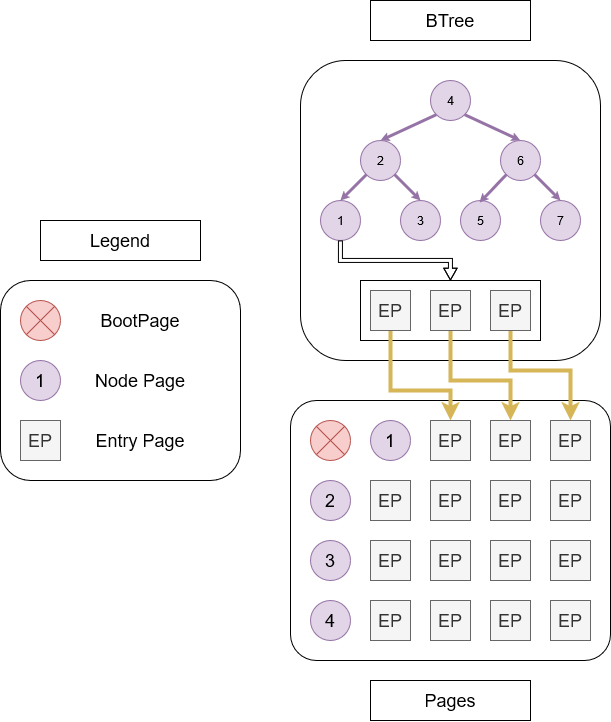
\includegraphics[width=.45\linewidth]{figures/Prototipo.png}
                \caption{Rappresentazione schematica del prototipo}
                \label{fig:prototipo}
            \end{figure}

        \subsection{Schema UML}

            Il sistema descritto precedentemente è stato modellato in un diagramma UML che ne riflette l’architettura logica e le relazioni tra componenti.

            Un diagramma UML è un tipo di diagramma strutturale che rappresenta un sistema o un processo attraverso una serie di elementi grafici, come classi, interfacce e relazioni.

            \begin{figure} [h]
                \centering
                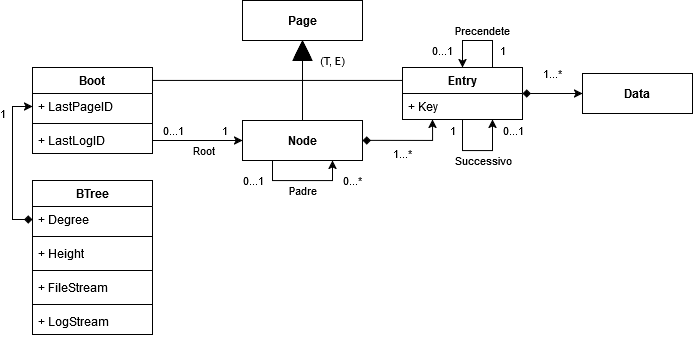
\includegraphics[width=1\linewidth]{figures/UML.png}
                \caption{Diagramma UML del prototipo}
                \label{fig:uml}
            \end{figure}

            Nel nostro diagramma, la classe \texttt{BTree} funge da mediatore tra la logica ad albero e la storicizazione dei dati, gestendo le operazioni di ricerca, inserimento e cancellazione.

            La classe \texttt{BTree} contiene inoltre riferimenti anche al file di Log il quale conterrà le modifiche di riferimento per i controlli di sicurezza.

            È presente inoltre una relazione di composizione tra la classe \texttt{BTree} e la classe \texttt{Boot}, che rappresenta la pagina iniziale all'interno del file di sotricizazione.

            La classe \texttt{Page} è una classe astratta che rappresenta una generica pagina all'interno del file di storicizzazione, e viene estesa dalle classi \texttt{Boot}, \texttt{Node} e \texttt{Entry}.

            Questa gerarchia favorisce il riuso del codice e l’isolamento delle responsabilità, riducendo l’accoppiamento tra logica di storage e operazioni sull’albero.

            In conclusione, l’adozione del \textit{BTree} come mediatore centralizza il flusso di controllo, semplificando l’aggiunta di nuove funzionalità, mentre la separazione tra Page e le sue implementazioni favorisce il riuso del codice e l’isolamento delle responsabilità, riducendo l’accoppiamento tra logica di storage e operazioni sull’albero.

    \section{Sviluppo}

        Segue ora una breve panoramica delle tecnologie utilizzate per lo sviluppo del prototipo.

        \subsection{Linguaggio di Programmazione}

            La scelta del linguaggio di programmazione è ricaduta su \texttt{C\#}, in quanto è il linguaggio che è già stato usato per il prodotto.

            \texttt{C\#} è un linguaggio versatile e performante, con un'ampia base di utenti e una vasta libreria standard.

            Inoltre, questo è particolarmente adatto per applicazioni di sistema, grazie alla sua portabilità, alla gestione della memoria automatica e alla robustezza.

        \subsection{Librerie}
        \label{subsec:Librerie}

            In aggiunta al linguaggio di programmazione è stato di notevolmente supporto l’impiego di diverse librerie, selezionate per implementare funzionalità specifiche e ottimizzare il flusso di lavoro.

            In particolare, tra le librerie della famiglia \texttt{System} si evidenziano:

            \begin{itemize}
                \item \textbf{Gestione dei File Binari:} È stata impiegata la libreria \texttt{System.IO}, che fornisce un insieme di funzionalità avanzate per la lettura e la scrittura di file in formato binario.

                Questo strumento si è rivelato fondamentale per operazioni che richiedono un elevato grado di precisione nella manipolazione dei dati non testuali, garantendo un accesso efficiente e sicuro alle informazioni archiviate.

                \item \textbf{Gestione delle Strutture Dati:} La libreria \texttt{Collections.Generic} è stata utilizzata per sfruttare un’ampia gamma di strutture dati predefinite, quali liste, code e dizionari.

                Queste strutture permettono una gestione dinamica e performante dei dati, facilitando l’implementazione di algoritmi complessi e contribuendo a mantenere l’ottimizzazione delle risorse di sistema.
            \end{itemize}

            Per la gestione e realizzazione dei test, invece si è fatto utilizzo della libreria \texttt{BenchmarkDotNet} e \texttt{XUnit}.

            La libreria \texttt{BenchmarkDotNet} è particolarmente apprezzata per le sue funzionalità avanzate nella misurazione delle performance del codice, offrendo strumenti di analisi dettagliata dei risultati.

            Ciò ha permesso di identificare in maniera accurata eventuali colli di bottiglia e di ottimizzare ulteriormente l’efficienza computazionale dell’applicazione.

        \subsection{Strumenti di Sviluppo}

            Per la realizzazione del prototipo, è stato adottato un insieme di strumenti di sviluppo che hanno contribuito significativamente alla qualità e all’efficienza del processo di implementazione. In particolare, si evidenziano:

            \begin{itemize}
                \item \textbf{Visual Studio}: È stato scelto come ambiente di sviluppo integrato per \textit{C\#}. \textit{Visual Studio} offre un ambiente completo e funzionale, caratterizzato da potenti strumenti per il debugging, l’analisi del codice e la gestione dei progetti.

                L’integrazione con altre tecnologie \textit{Microsoft} ha permesso di accelerare le fasi di codifica e testing, contribuendo in modo determinante alla qualità del software prodotto.

                \pagebreak

                \item \textbf{Git}: Per il controllo versione del codice, si è fatto ricorso a \textit{Git}, un sistema distribuito che consente di tracciare tutte le modifiche apportate durante lo sviluppo.

                Git ha facilitato la gestione della cronologia del progetto, permettendo di sperimentare modifiche in modo sicuro e coordinato, e di supportare un lavoro collaborativo efficace all'interno del team.

                \item \textbf{GitHub}: Come piattaforma di hosting per progetti basati su \textit{Git}, \textit{GitHub} ha offerto un ambiente collaborativo per la condivisione del codice e la gestione delle versioni.
            \end{itemize}

            L'integrazione di questi strumenti ha permesso di adottare un approccio allo sviluppo più dinamico e assicurando una gestione ottimale del ciclo di vita del software.

        \subsection{Sviluppo del Sistema di Serializzazione e Deserializzazione}

            La prima fase dello sviluppo del prototipo ha riguardato la progettazione e l’implementazione di un sistema dedicato alla serializzazione e deserializzazione dei dati.

            L’obiettivo era quello di sostituire il formato \textit{MessagePack}, attualmente in uso, con un formato binario ottimizzato, capace di ridurre la dimensione dei dati e di semplificare le operazioni di lettura e scrittura.

            In una fase preliminare era già stata affrontata la problematica dell’eterogeneità dei dati attraverso la definizione di un formato univoco per i dati da storicizzare.

            Pertanto, il focus di questa fase si è concentrato sulla riduzione dell’overhead e sul perfezionamento del processo di serializzazione.

            Per raggiungere questi obiettivi sono state adottate le seguenti strategie:
            \begin{itemize}
                \item \textbf{Calcolo della Dimensione degli Elementi:} È stato effettuato un calcolo accurato della dimensione di ogni singolo elemento del pacchetto dati, in modo da poter dimensionare in modo preciso l’allocazione dello spazio su di uno Stream binario.
                \item \textbf{Utilizzo di Tipi a Lunghezza Fissa:} Dove possibile, sono stati impiegati tipi a lunghezza fissa per rappresentare i dati, standardizzando la codifica e minimizzando l’impatto sullo spazio occupato.
            \end{itemize}

            Il risultato di questo approccio è stato la definizione di un formato binario altamente efficiente, capace di ridurre la dimensione complessiva dei dati serializzati di circa il 60\% rispetto a \textit{MessagePack}, pur mantenendo prestazioni comparabili in termini di tempistiche di lettura e scrittura.

            A dimostrazione dell'efficienza di questo formato è stato condotto un test di benchmarking, che ha confermato la riduzione della dimensione dei dati serializzati e l'ottimizzazione delle prestazioni.

            \begin{figure} [h]
                \centering
                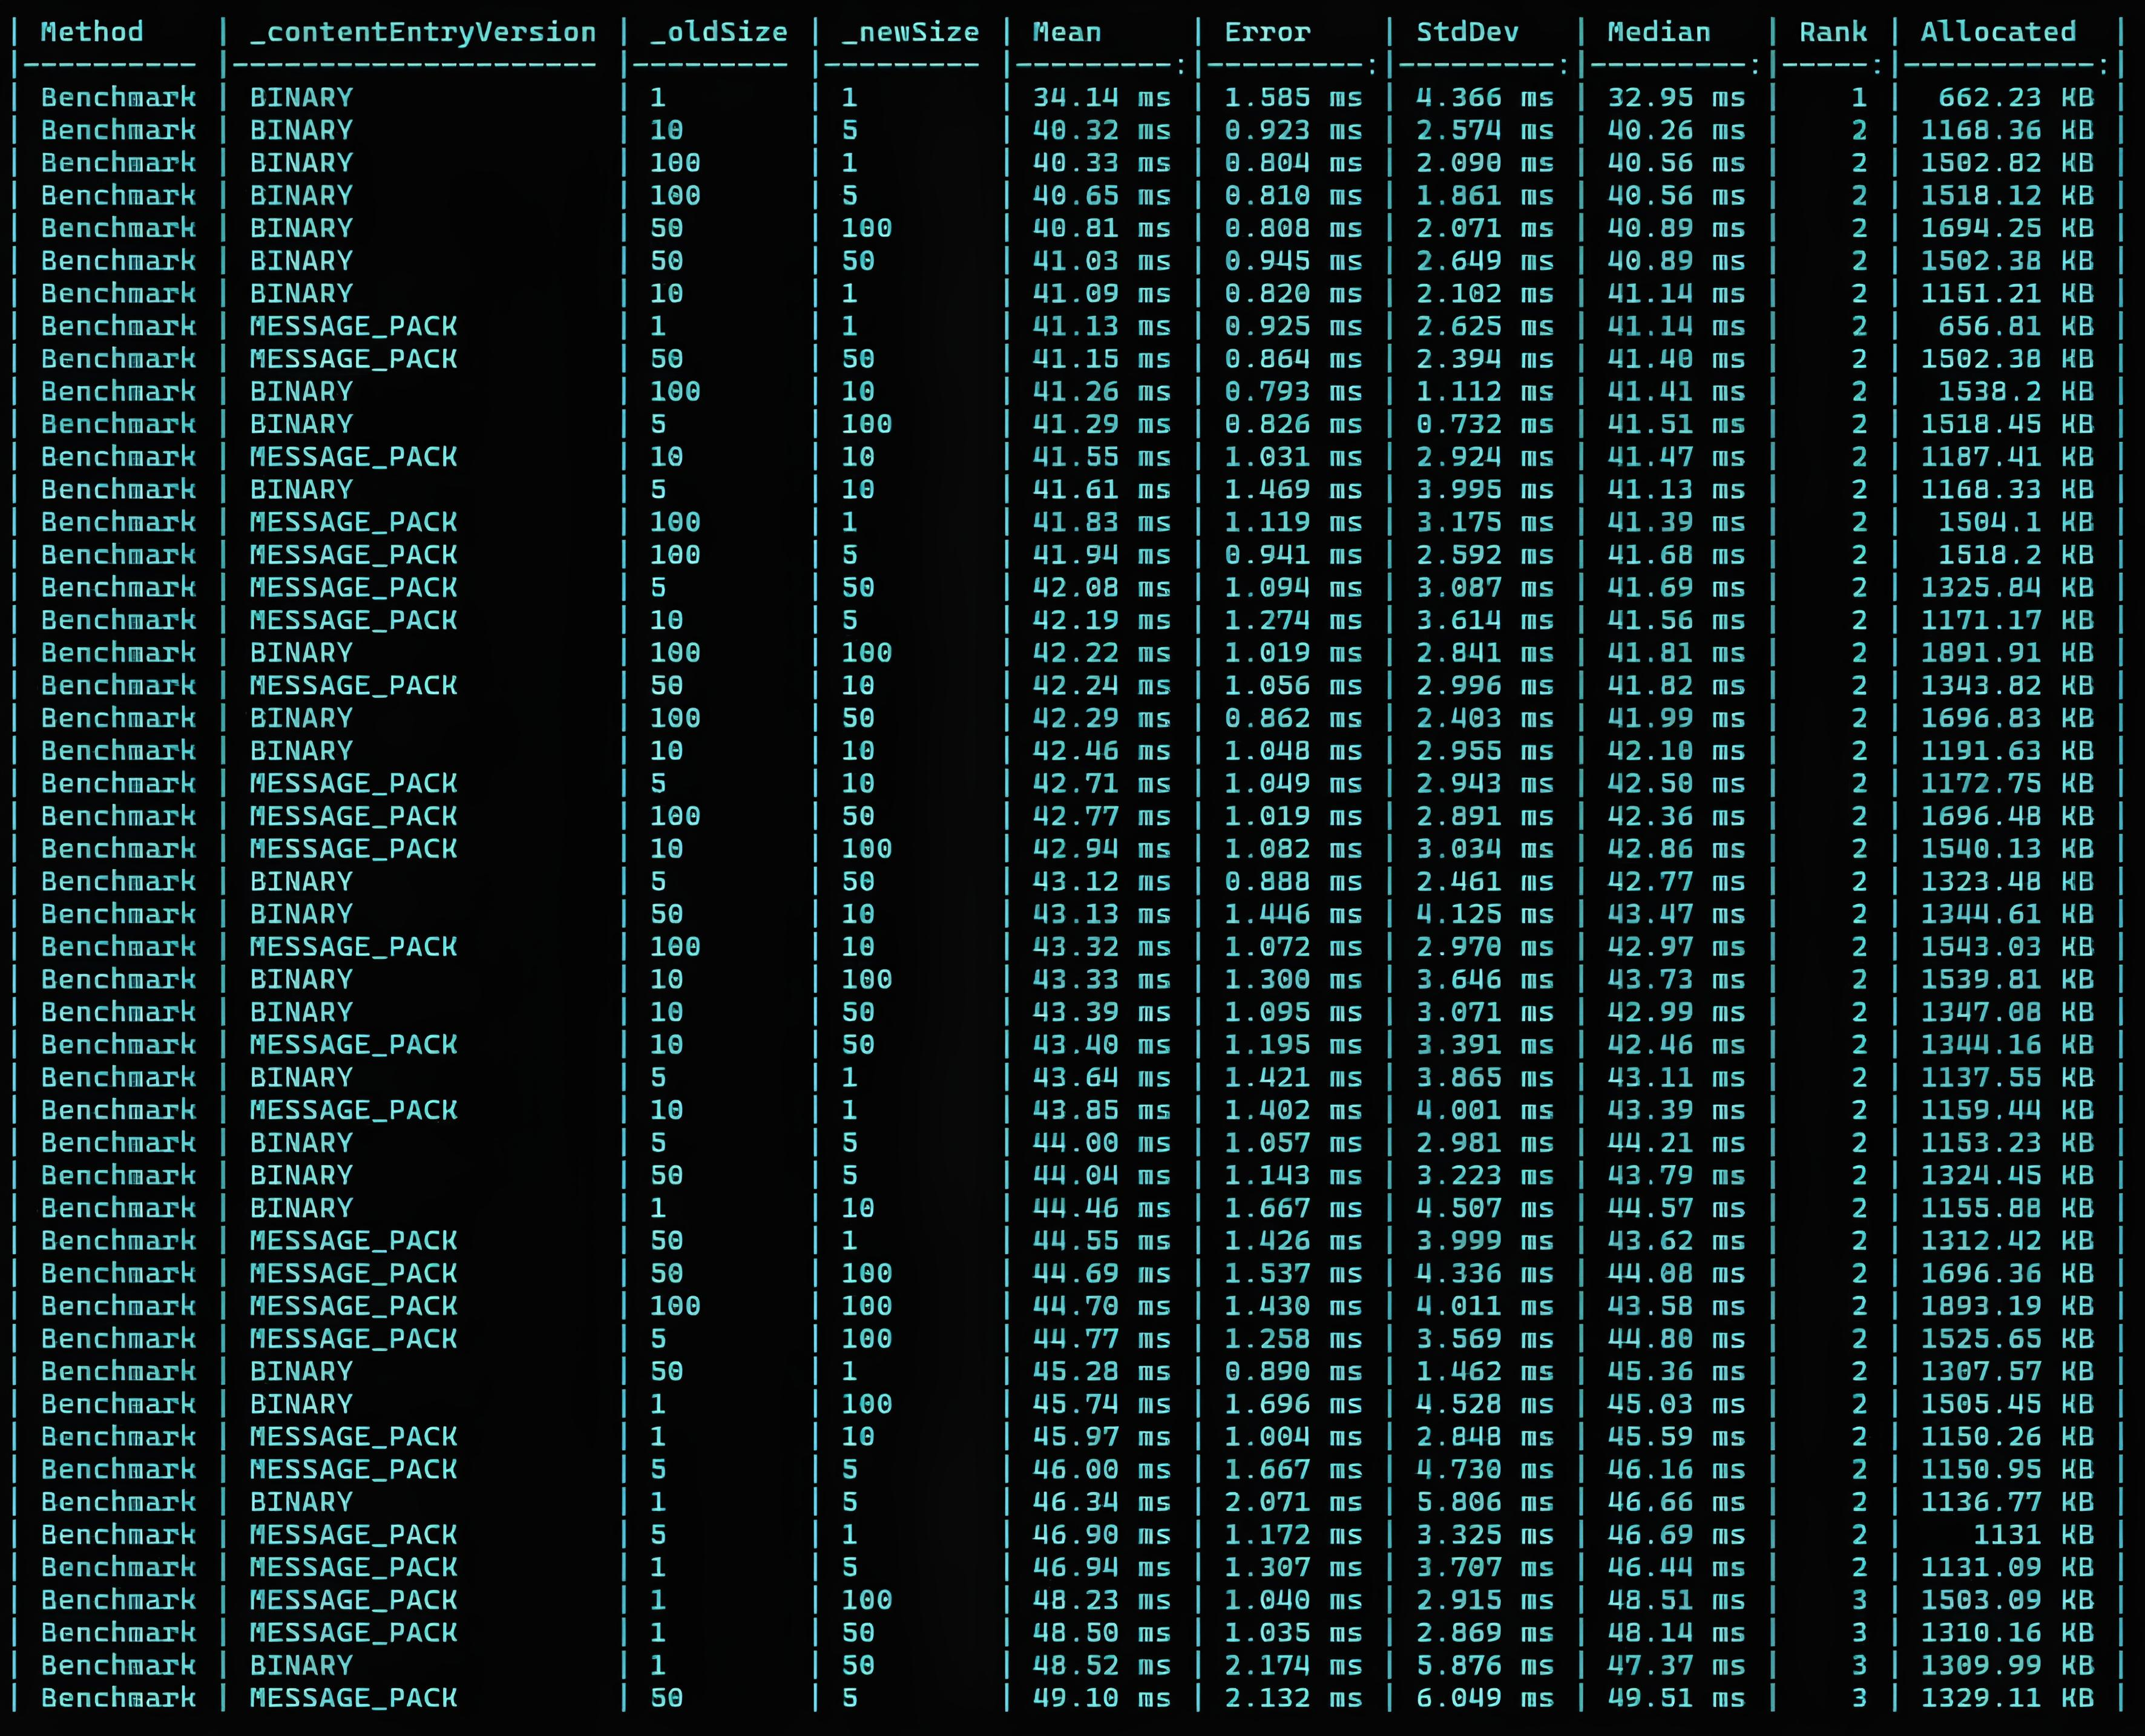
\includegraphics[width=1\linewidth]{figures/BenchmarkS-D.jpeg}
                \caption{Risultati del Benchmarking}
                \label{fig:serialization}
            \end{figure}

        \clearpage

        \subsection{Realizzazione del Btree}

            La fase successiva dello sviluppo ha riguardato la progettazione e la realizzazione del \textit{B-Tree}, che ha rappresentato il nucleo centrale del prototipo sviluppato.

            Questa sezione descrive le soluzioni implementate per garantire un bilanciamento efficiente tra prestazioni e persistenza dei dati.

            \subsubsection{Analisi Preliminare e Riferimenti Teorici}

                Il processo di sviluppo è iniziato con un'analisi approfondita dello pseudocodice del \textit{B-Tree}, tratto dal testo accademico \textbf{Introduction to Algorithms} \cite{cormen2022introduction}.

                Lo studio ha permesso di comprendere e integrare concetti fondamentali quali:
                \begin{itemize}
                    \item Le politiche di \textit{Suddivisione}(o \textit{Splitting}) e \textit{Fusione} (o \textit{Merging}) dei nodi.
                    \item Le strategie di ricerca delle chiavi all'interno della struttura.
                    \item I vincoli tecnici imposti dall'albero per garantire un bilanciamento efficiente.
                \end{itemize}

                A partire da questa analisi, sono state identificate le classi e i metodi necessari per la realizzazione del \textit{B-Tree}, delineando le interfacce e le relazioni tra i vari componenti del sistema.

                Una volta definite le caratteristiche principali della struttura dati, si è passati alla fase di implementazione.

            \subsubsection{Implementazione e adattamento del codice}

                In questa fase sono state sviluppate le classi e i metodi necessari per la gestione delle operazioni fondamentali del \textit{B-Tree}, tra cui ricerca, inserimento e cancellazione delle chiavi, assicurando il rispetto delle proprietà strutturali dell’albero.

                Come base per l’implementazione, è stato adottato il codice \textit{open-source} \texttt{btree dotnet} \cite{rsdcastro_btree_dotnet}, un’implementazione in \texttt{C\#} che forniva lo scheletro delle classi e delle operazioni principali.

                Tuttavia, la libreria presentava alcune criticità: non era compatibile con le versioni più recenti del linguaggio e conteneva errori nel meccanismo di bilanciamento dell’albero durante la fase di rimozione.

                Per superare queste problematiche, è stato necessario apportare modifiche significative al codice, convalidandole successivamente attraverso una serie di test di controllo per garantire la correttezza e la stabilità del sistema.

            \subsubsection{Implementazione delle Page}

                Successivamente, si è proceduto allo sviluppo delle \texttt{Page} e delle loro specifiche estensioni: \texttt{BootPage}, \texttt{NodePage} e \texttt{EntryPage}.

                \lstinputlisting[float,language=csh,label={lst:Page}]{listings/BTree/Page.cs}

                La classe \texttt{Page} rappresenta una pagina di memoria persistente, un elemento tipico dei sistemi di storage su file, come quelli utilizzati nei database.

                Questa classe è progettata per rispettare una serie di caratteristiche fondamentali, indispensabili per garantire la corretta gestione dei dati.

                Attributi:
                \begin{itemize}
                    \item \textbf{\texttt{ID}}: Un identificatore univoco della \texttt{Page} all'interno del file.
                    \item \textbf{\texttt{Type}}: Un codice identificativo che specifica il tipo della pagina, distinguendo le varie specializzazioni.
                    \item \textbf{\texttt{Buffer}}: Un array di byte che contiene il contenuto memorizzato nella pagina.
                    \item \textbf{\texttt{FreePageSize}}: Un indicatore della quantità di spazio libero disponibile all'interno della pagina.
                    \item \textbf{\texttt{IsModified}}: Una flag di controllo che segnala eventuali modifiche apportate alla pagina, fondamentale per le operazioni di storicizzazione e sincronizzazione dei dati.
                \end{itemize}

                Metodi:
                \begin{itemize}
                    \item \textbf{\texttt{Read}}: Metodo per la lettura dei dati dal buffer della pagina, che aggiorna contestualmente i vari campi per garantire la coerenza delle informazioni.
                    \item \textbf{\texttt{Write}}: Metodo responsabile della scrittura dei dati nel buffer, assicurando che le modifiche vengano correttamente registrate e mantenute.
                \end{itemize}

            \subsubsection{Sviluppo della BootPage}

                La classe \texttt{BootPage}, introdotta come primo componente specializzato del sistema, funge da interfaccia primaria per la gestione delle pagine all’interno di un file.

                Inoltre, tale pagina si occupa in modo centrale di orchestrare il riutilizzo degli spazi liberi presenti all’interno del file, garantendo così una gestione efficiente della memoria e un’ottimizzazione delle operazioni di I/O.

                \lstinputlisting[float,language=csh,label={lst:BootPage}]{listings/BTree/BootPage.cs}

                Attributi:
                \begin{itemize}
                    \item \textbf{\texttt{LastPageID}}: Un indice che indica l’ultima pagina aggiunta alla fine del file, fungendo da riferimento per l’espansione del file stesso.
                    \item \textbf{\texttt{LastLogVersionID}}: Un Indice che rappresenta la versione corrente del log del sistema, fondamentale per il tracciamento delle operazioni eseguite.
                    \item \textbf{\texttt{Buffer}}: Un array di byte che contiene la trascrizione del contenuto della pagina, utilizzato per la lettura e la scrittura dei dati.
                    \item \textbf{\texttt{EmptyPageIndexes}}: Una lista degli indici relativi alle pagine vuote presenti nel file.
                    Questi spazi vengono prioritariamente riutilizzati, evitando così la creazione non necessaria di nuove pagine.
                    \item \textbf{\texttt{RootPageID}}: L'indice della radice del nostro albero, che rappresenta il punto iniziale di riferimento per l’organizzazione delle altre pagine.
                \end{itemize}

                Metodi:
                \begin{itemize}
                    \item \textbf{\texttt{AddID}}: Metodo responsabile dell’aggiunta di un nuovo \texttt{ID} alla lista di indici liberi, aggiornando così il set di pagine disponibili per il riutilizzo.
                    \item \textbf{\texttt{GetNewPageID}}: Metodo che gestisce la generazione di un nuovo \texttt{PageID}.
                    Se sono presenti pagine vuote (già indicate in \texttt{EmptyPageIndexes}), il metodo ne effettua il riutilizzo.
                    In assenza di queste, ne viene creato uno nuovo.
                    \item \textbf{\texttt{GetNewLogID}}: Metodo dedicato alla generazione di un nuovo \texttt{LogID}, aggiornando la versione del log e contribuendo al mantenimento della consistenza del sistema.
                \end{itemize}

            \subsubsection{Sviluppo della NodePage}

                Successivamente, la classe \texttt{Node} dell'albero è stata riadattata nella forma di Page nella classe \texttt{NodePage}, apportando modifiche sia ai metodi che agli attributi per integrarsi al meglio nel nuovo sistema basato su pagine.

                Questa trasformazione ha portato alla suddivisione del codice in due sezioni distinte.

                La prima sezione illustra come vengono gestiti i nodi figli all'interno di una \texttt{NodePage}. Oltre alle operazioni classiche di aggiunta, rimozione e ricerca, è stata implementata la funzione di controllo validità \texttt{CheckChildPage}. Questo metodo esegue controlli specifici per verificare la correttezza dei puntatori ai nodi figli, prevenendo così errori di accesso e garantendo la coerenza strutturale.

                Mentre la seconda sezione rappresenta il sistema di gestione delle entry contenute nella \texttt{NodePage}. Analogamente a quanto avviene per i nodi figli, anche qui è stata integrata una funzione di controllo validità, \texttt{CheckEntryPage}, che verifica l'integrità delle entry e assicura la correttezza dei dati gestiti.

                \lstinputlisting[float=h,language=csh,label={lst:NodePageChildSection}]{listings/BTree/NodePageChildSection.cs}

                \lstinputlisting[float=h,language=csh,label={lst:NodePageEntrySection}]{listings/BTree/NodePageEntrySection.cs}

                \clearpage

            \subsubsection{Sviluppo della EntryPage}

                Infine, è stata sviluppata la classe \texttt{EntryPage}, che rappresenta l'unità fondamentale dello storage del sistema.

                Questa classe è progettata per gestire in maniera efficiente la memorizzazione e la manipolazione dei dati, garantendo che ogni operazione sullo storage venga eseguita in modo ordinato e affidabile.

                I principali elementi di interesse di questa classe sono le 3 funzioni di gestione dei dati all'interno della \texttt{EntryPage}.

                \begin{itemize}
                    \item \textbf{\texttt{AddData}}: Metodo dedicato all'aggiunta di nuovi dati nella \texttt{EntryPage}.
                    Questo metodo assicura che i dati vengano inseriti correttamente all'interno della struttura, aggiornando opportunamente lo stato della pagina.
                    \item \textbf{\texttt{SetData}}: Metodo che, a partire da una struttura enumerabile, consente la modifica dei dati presenti nella \texttt{EntryPage}.
                    Questa funzione garantisce che le modifiche vengano applicate in modo coerente e affidabile, mantenendo la consistenza dei dati.
                    \item \textbf{\texttt{FindPositionToInsert}}: Metodo incaricato di determinare la posizione ottimale in cui inserire un nuovo dato. Questo approccio garantisce una distribuzione equilibrata dei dati all'interno della pagina e contribuisce a ottimizzare l'utilizzo dello spazio disponibile.
                \end{itemize}

                \lstinputlisting[float,language=csh,label={lst:EntryPage}]{listings/BTree/EntryPage.cs}

                \clearpage

            \subsubsection{Sviluppo della classe BTree}

                Come ultima classe del sistema è stata sviluppata la classe \texttt{BTree}, che rappresenta il mediatore tra la logica ad albero e la storicizazione dei dati, gestendo le operazioni di ricerca, inserimento e cancellazione.

                \paragraph{Creazione degli Elementi del BTree}

                    La successiva sezione di codice illustra come vengono creati gli elementi fondamentali del \texttt{BTree}: la radice, i nodi e le entry, che costituiscono la struttura portante del sistema.

                    \begin{itemize}
                        \item \textbf{\texttt{CreateNewRoot}}: Crea una nuova radice dell'albero generando una nuova istanza di \texttt{NodePage} con un ID univoco ottenuto dalla \texttt{BootPage}.
                        Dopo la creazione, aggiorna l'ID della radice nel \texttt{BootPage} e aggiunge quest'ultimo alle collezioni di pagine loggate e bufferizzate.
                        \item \textbf{\texttt{CreateNewNode}}: Genera un nuovo nodo non radice creando un'istanza di \texttt{NodePage} con un nuovo ID.
                        Anche in questo caso, il \texttt{BootPage} viene registrato nelle collezioni di log e buffer prima della creazione del nodo.
                        \item \textbf{\texttt{CreateNewEntry}}: Crea una nuova entry (istanza di \texttt{EntryPage}) per memorizzare una chiave specificata.
                        Viene ottenuto un nuovo ID dalla \texttt{BootPage}, e il nuovo oggetto viene inizializzato con i parametri necessari, mentre alcuni valori sono impostati su \texttt{null}.
                        Anche qui, la \texttt{BootPage} viene aggiunta alle strutture di log e buffer.
                    \end{itemize}

                    Questi metodi garantiscono la corretta generazione e registrazione di nuovi elementi (radice, nodi e entry) all'interno della struttura, mantenendo la coerenza delle collezioni di pagine loggate e bufferizzate.

                    \lstinputlisting[float,language=csh,label={lst:BTreeElementsCreation}]{listings/BTree/BTreeElementsCreation.cs}

                    \clearpage

                \paragraph{Metodi per l'inserimento nel BTree}

                    Questo frammento di codice mostra l'implementazione del metodo di inserimento di un nuovo elemento all'interno del BTree seguendo questi passaggi principali:

                    \begin{itemize}
                        \item \textbf{Inserimento nella radice non piena}: Se il nodo radice ha ancora spazio, la chiave e i dati vengono inseriti direttamente usando un metodo ricorsivo che, nel caso di nodo foglia, crea una nuova entry, oppure, se il nodo non è foglia, individua il figlio appropriato per continuare l'inserimento.
                        \item \textbf{Gestione del nodo radice pieno}: Se la radice è piena, viene creata una nuova radice; il vecchio nodo radice viene aggiunto come figlio della nuova radice e suddiviso (split) per mantenere l'equilibrio dell'albero. Successivamente, si procede con l'inserimento ricorsivo nella nuova struttura.
                        \item \textbf{Aggiornamenti e persistenza}: Dopo ogni inserimento, vengono aggiornati il log, la cache dei nodi modificati e viene eseguita la serializzazione dell'albero per garantire consistenza e persistenza dei dati.
                    \end{itemize}

                    Questo approccio assicura che l'albero rimanga bilanciato, consentendo operazioni di ricerca e inserimento efficienti.

                    \lstinputlisting[float,language=csh,label={BTreeInsert}]{listings/BTree/BTreeInsert.cs}

                    \clearpage

                \paragraph{Metodi per la rimozione nel BTree}

                    Segue ora una descrizione dei metodi implementati per la rimozione degli elementi dal \texttt{BTree}.

                    Il metodo \texttt{Delete} avvia il primo passo del processo di eliminazione a partire dalla radice dell'albero.

                    Dopo aver eseguito l'eliminazione, verifica se la radice è diventata vuota e non è una foglia; in tal caso, la sostituisce con il suo primo figlio e decrementa l'altezza dell'albero. Successivamente, aggiorna il log, scrive i contenuti dei buffer e serializza la struttura per garantire la persistenza dei dati.

                    \lstinputlisting[float=h,language=csh,label={BTreeDelete}]{listings/BTree/BTreeDelete.cs}

                    Il metodo \texttt{DeleteInternal} cerca la posizione della chiave da eliminare nel nodo corrente confrontandola con le chiavi presenti.

                    Se la chiave viene trovata nel nodo, chiama il metodo DeleteKeyFromNode per gestire l'eliminazione.

                    Se il nodo non è una foglia e la chiave non è presente, propaga l'eliminazione al sottoalbero appropriato, corrispondente all'intervallo di chiavi.

                    \lstinputlisting[float=h,language=csh,label={BTreeDeleteInternal}]{listings/BTree/BTreeDeleteInternal.cs}

                    \clearpage

                    Infine, il metodo \texttt{DeleteKeyFromNode} gestisce diversi scenari.

                    Se il nodo è una foglia, rimuove direttamente la chiave.

                    Se è un nodo interno, tenta di sostituire la chiave con il predecessore, la chiave massima del sottoalbero sinistro, se il figlio sinistro ha un numero di elementi maggiore o uguale al grado dell'albero.

                    Se ciò non è possibile, prova con il successore, la chiave minima del sottoalbero destro, se il figlio destro ha sufficienti elementi.

                    Se entrambi i figli hanno meno di \texttt{Degree} elementi, fonde il nodo corrente con i suoi figli e propaga l'eliminazione nel nodo risultante, mantenendo così le proprietà del \texttt{B-Tree}.

                    \lstinputlisting[float=h,language=csh,label={BTreeDeleteKeyFromNode}]{listings/BTree/BTreeDeleteKeyFromNode.cs}

                \pagebreak

                \paragraph{Metodi per la ricerca nel BTree}

                    Il metodo di ricerca in un \texttt{B-tree} permette di localizzare un elemento specifico all'interno dell'albero attraverso la sua chiave identificativa.

                    Questo processo si basa su una strategia ricorsiva che sfrutta l'organizzazione ordinata delle chiavi presenti nella struttura.

                    L'implementazione di tale metodo è strutturata in due metodi distinti: uno pubblico, che funge da punto di accesso esterno e avvia la ricerca a partire dal nodo radice dell'albero, e uno ricorsivo interno, incaricato di gestire l'atraversamento dei nodi e il percorso gerarchico all'interno della struttura.

                    La ricerca si articola in diverse fasi, ciascuna finalizzata a individuare la posizione corretta della chiave all'interno dell'albero.

                    Inizialmente, viene effettuata un'analisi del nodo corrente, l'obiettivo è determinare quante di queste chiavi presenti nel nodo risultano essere inferiori rispetto alla chiave che si sta cercando.

                    Tale conteggio permette di identificare l'indice del sottoalbero in cui la ricerca dovrà proseguire.

                    Contemporaneamente, si verifica se una delle chiavi presenti nel nodo corrente corrisponde esattamente alla chiave target. In caso affermativo, la ricerca si conclude con successo e l'elemento viene immediatamente restituito.

                    Qualora il nodo in esame sia una foglia, ovvero un nodo terminale dell'albero privo di ulteriori diramazioni, e la chiave non sia presente, la ricerca termina con un esito negativo, segnalando l'assenza dell'elemento attraverso la restituzione di un valore nullo.

                    Se, al contrario, il nodo non è una foglia, la ricerca prosegue in modo ricorsivo.

                    Viene selezionato il figlio corrispondente all'indice precedentemente calcolato e la funzione di ricerca viene richiamata su tale figlio, ripetendo il processo.

                    La natura ricorsiva dell'algoritmo garantisce una scansione completa dell'albero in profondità, fino a raggiungere un nodo foglia o a individuare una corrispondenza con la chiave cercata.

                    L'efficienza di questa operazione è notevole: grazie alla struttura bilanciata del B-tree, la ricerca ha una complessità logaritmica, proporzionale al logaritmo del numero totale di elementi presenti nell'albero.

                    \pagebreak

                    La terminazione dell'algoritmo è sempre garantita: la ricerca raggiunge inevitabilmente un nodo foglia o identifica una corrispondenza, escludendo la possibilità di cicli infiniti.

                    \lstinputlisting[float=h,language=csh,label={BTreeSearch}]{listings/BTree/BTreeSearch.cs}

                \paragraph{Metodi di Utility del BTree}

                    Lo \texttt{Split}, e la sua controparte \texttt{Merge}, sono operazioni critiche attive durante l'inserimento (o l'eliminazione) di nuove chiavi, quando un nodo supera la capacità massima (o minima) definita dal \textit{Grado} dell'albero.

                    Queste procedure preservano l'equilibrio strutturale del \texttt{B-tree}, condizione essenziale per le prestazioni logaritmiche.

                    A differenza delle operazioni di \texttt{Merge}, che sono state già integrate all'interno delle operazioni di eliminazione, lo \texttt{Split} è stato implementato come metodo autonomo.

                    \clearpage

                    \lstinputlisting[float=h,language=csh,label={BTreeSplit}]{listings/BTree/BTreeSplit.cs}

                    Il processo si articola in cinque fasi:
                    \begin{enumerate}
                        \item \textbf{Creazione di un nuovo nodo}: Viene allocato un nodo ausiliario per ospitare una porzione delle chiavi.
                        \item \textbf{Promozione della chiave mediana}: La chiave centrale del nodo saturo viene spostata nel nodo genitore, agendo da separatore.
                        \item \textbf{Collegamento del nuovo nodo}: Il nodo creato viene associato al genitore come figlio destro della chiave promossa.
                        \item \textbf{Ridistribuzione delle chiavi}: Le chiavi successive alla mediana vengono riposizionate all'interno del nuovo nodo, lasciando il nodo originale con \textit{Grado - 1} elementi.
                        \item \textbf{Gestione dei figli (per nodi non foglia)}: Se il nodo splittato non è una foglia, i puntatori ai figli vengono ripartiti tra nodo originale e nuovo nodo, mantenendo la corretta gerarchia.
                    \end{enumerate}

                    Al termine, i metadati dei nodi coinvolti (genitore, nuovo nodo e nodo originale) vengono aggiornati per riflettere la nuova configurazione.

                    Lo \texttt{Split} garantisce così una crescita controllata dell'albero, prevenendo sbilanciamenti e assicurando che tutte le operazioni mantengano una complessità logaritmica.

                \paragraph{Metodi di Serializzazione e Deserializzazione del BTree}

                    L'atto di seriallizare ha lo scopo di rendere persistenti i dati, su un supporto di memorizzazione di massa (come un disco).

                    Questo processo avviene attraverso due fasi distinte: la prima fase riguarda la scrittura di un log, mentre la seconda fase si concentra sul salvataggio effettivo dei dati.

                    Nella fase iniziale, dedicata alla scrittura del log, il metodo itera sull'insieme delle \texttt{Page} contenute in una lista.

                    Per ciascuna di queste \texttt{Page}, viene creato un array di byte di dimensione fissa. Successivamente, il viene chiamato il metodo Write della pagina che provvede a popolare questo array con i dati specifici della pagina L'array così ottenuto viene poi scritto nel flusso di log.

                    Qualora si verifichi un errore durante questa fase di scrittura, viene generata un'eccezione, accompagnata dal messaggio ``Unable to create a new log".

                    Una volta completata la scrittura di tutte le pagine di log, lo stream viene chiuso attraverso il metodo Dispose.

                    Successivamente, il codice tenta di aprire un nuovo file di log, utilizzando un percorso che combina la cartella di destinazione con un identificativo di log univoco, ottenuto attraverso la \texttt{BootPage}.

                    Dopo la scrittura e la riapertura del file di log, la lista di \texttt{Page} viene ricreata come una nuova istanza vuota.

                    Questa operazione ha lo scopo di liberare la memoria precedentemente occupata dalle pagine di log che sono state salvate.

                    \pagebreak

                    La seconda fase del processo di serializzazione prevede la scrittura effettiva dei dati. In questa fase, il metodo itera sull'insieme delle pagine presenti nella lista di \texttt{Page} da serializzare.

                    Analogamente alla fase precedente, per ciascuna pagina viene creato un array di byte della dimensione predefinita, e la pagina stessa provvede a scrivere i propri dati all'interno di questo array.

                    Prima di scrivere definitivamente i dati nell'array, è fondamentale che il flusso di dati sia allineato con precisione a un punto specifico del file. Questo garantisce che le informazioni vengano memorizzate nella posizione corretta e che possano essere recuperate in modo accurato in seguito.

                    Qualora si verifichi un errore durante questa fase di scrittura, viene generata un'eccezione con il messaggio ``Unable to create a new save".

                    Una volta completato il salvataggio di tutte le pagine, anche la lista di \texttt{Page} da serializzare viene ricreata come una nuova istanza vuota, preparandolo per future operazioni di buffering.

                    \lstinputlisting[float=h,language=csh,label={BTreeSerialize}]{listings/BTree/BTreeSerialize.cs}

                    \clearpage

                    Nel caso della deserializzazione poniamo particolare interesse sulla deserializzazione delle \texttt{Entry}. Il metodo \texttt{DeserializeEntryFromID} ha proprio questo specifico compito. In altre parole, trasforma una sequenza di byte letta dal disco in un oggetto \texttt{EntryPage} utilizzabile in memoria.

                    Il processo inizia con il posizionamento del cursore di lettura all'interno del file.

                    Il metodo riceve un ID come parametro e lo utilizza per calcolare l'offset, ovvero la posizione precisa nel file dove si trovano i dati della pagina desiderata.

                    Una volta posizionati nel punto giusto del file, si procede con la lettura dei dati.

                    Viene creato un array di byte, chiamato buffer, con una dimensione pari a quella di una pagina.

                    Successivamente, il metodo legge esattamente un quantitativo di byte dal file pari alla dimensioni di una \texttt{Page}, a partire dalla posizione corrente del puntatore, e li memorizza all'interno del buffer.

                    Dopo aver recuperato i dati dal file, è necessario verificarne il contenuto per assicurarsi che corrispondano al formato di una pagina di tipo \texttt{Entry}. Se la verifica ha successo, il metodo crea una nuova istanza dell'oggetto \texttt{EntryPage}.

                    \lstinputlisting[float=h,language=csh,label={BTreeDeserialize}]{listings/BTree/BTreeDeserialize.cs}

        \pagebreak

        \subsection{Sviluppo dei Test}

            Come precedentemente accennato nella \cref{subsec:Librerie}, per la gestione e realizzazione dei test si è fatto utilizzo della libreria \texttt{XUnit}.

            Grazie a questa libreria è stato possibile sviluppare una serie di test mirati e automatizzati, che hanno permesso di verificare la correttezza e l'efficienza del sistema.

            In particolare, sono stati sviluppati test per verificare il corretto funzionamento delle operazioni di inserimento, ricerca ed eliminazione delle chiavi all'interno del \texttt{B-Tree}.

            Per validare tali risultati sono stati realizzati diversi metodi di test, ciascuno focalizzato su un aspetto specifico del sistema. Esempio di questi controlli di validazione sono i test \texttt{ValidateTree} e \texttt{ValidateSubtree}.

            Il metodo \texttt{ValidateTree} avvia la validazione dall'albero, raccogliendo le chiavi presenti in un dizionario e verificando che coincidano con quelle attese, senza duplicati.

            Mentre \texttt{ValidateSubtree} opera in modo ricorsivo, controllando che ogni nodo, eccetto la radice, abbia:

            \begin{itemize}
                \item Il numero delle chiavi compreso nei limiti del BTree.
                \item Le chiavi ordinate correttamente entro intervalli specifici.
                \item I nodi interni contengano il numero minimo di figli richiesto.
            \end{itemize}

            In sostanza, il codice assicura che l'albero rispetti le proprietà strutturali e l'ordinamento tipico di un \texttt{B-Tree}.

            \lstinputlisting[float=h,language=csh,label={lst:ValidateTree}]{listings/Test/ValidateTree.cs}

            \clearpage

            Inoltre, sono stati sviluppati test di stress per valutare le prestazioni del sistema in condizioni generiche, verificando la capacità del \texttt{B-Tree} di gestire qualsiasi combinazione di inserimenti e eliminazioni.

            Il principale test per dimostrare ciò è il RunBruteForce. Il codice esegue un test brute force su un \texttt{B-Tree} del grado scelto. Procede con l'eseguire, per 1000 iterazioni, operazioni casuali di inserimento o cancellazione.

            Dopo ogni operazione, viene chiamato il metodo \texttt{CheckNode}, che attraversa ricorsivamente ogni nodo per controllare che, se ci sono figli, il loro numero sia esattamente quello atteso e che né il numero di chiavi né quello dei figli superino i limiti imposti dal grado.

            \lstinputlisting[float,language=csh,label={lst:BruteForce}]{listings/Test/BruteForce.cs}

\chapter{Conclusioni}

    \section{Risultati e Valutazioni}
        Il prototipo sviluppato ha dimostrato di essere un sistema efficiente e scalabile per la gestione di grandi quantità di dati, garantendo prestazioni elevate e una gestione ottimale delle risorse.

        Per dimostrazione, sono stati implementati vari benchmark che ci hanno permesso di ottenere le valutazioni desiderate. In ciascun benchmark, all'inizio di ogni iterazione viene creato un B-Tree di grado \textit{n} contenente \text{m} chiavi.

        Successivamente, per ogni combinazione di \text{n} e \text{m} vengono eseguite diverse operazioni—come inserimento, cancellazione e ricerca di un elemento—per valutarne le prestazioni.

        Da questi benchmark sono stati poi estratti i seguenti risultati:

        \begin{figure} [h]
            \centering
            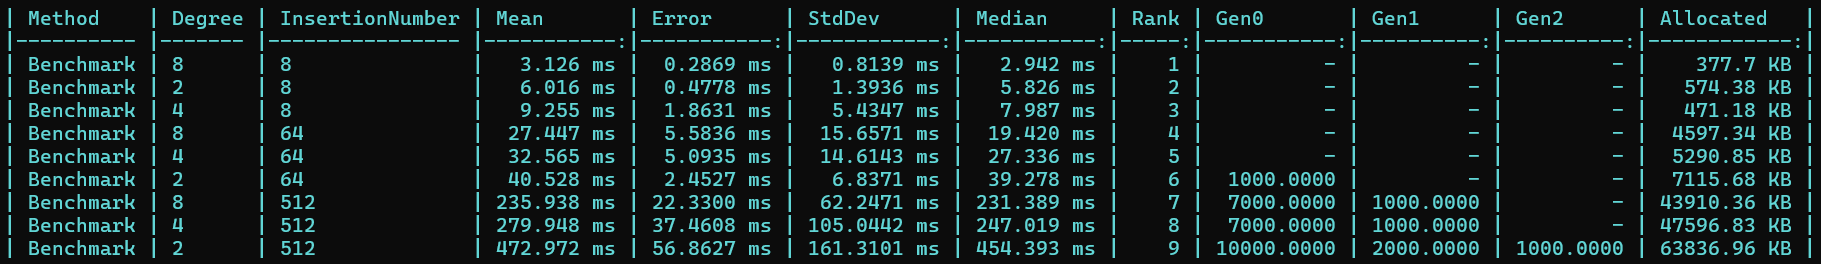
\includegraphics[width=1\linewidth]{figures/BenchmarkInsertion.png}
            \caption{Risultati del Benchmarking dell'inserimento}
            \label{fig:benchmarkA}
        \end{figure}

        \begin{figure} [h]
            \centering
            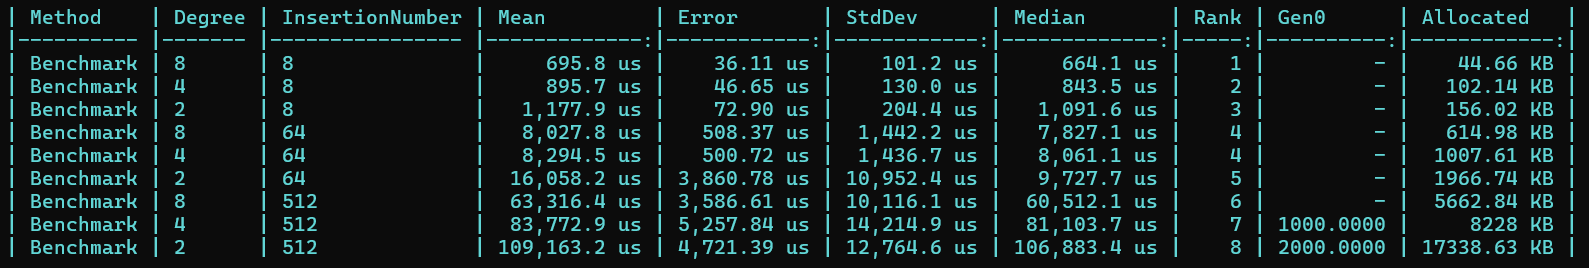
\includegraphics[width=1\linewidth]{figures/BenchmarkDelete.png}
            \caption{Risultati del Benchmarking dell'eliminazione}
            \label{fig:benchmarkB}
        \end{figure}

        \begin{figure} [h]
            \centering
            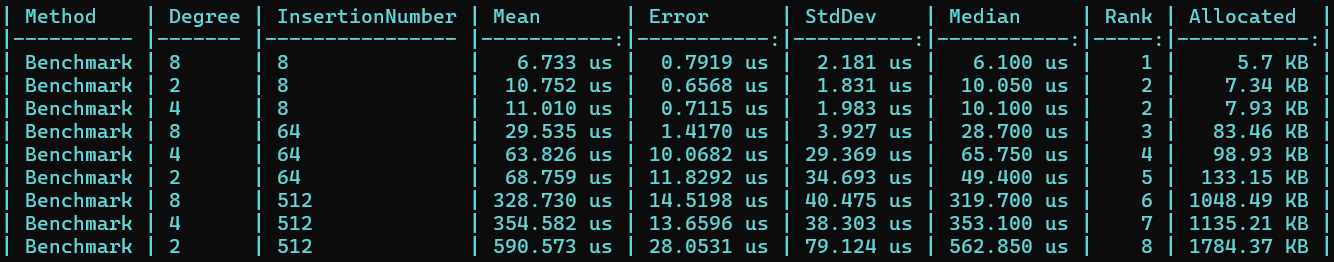
\includegraphics[width=1\linewidth]{figures/BenchmarkSearch.png}
            \caption{Risultati del Benchmarking della ricerca}
            \label{fig:benchmarkC}
        \end{figure}

        \clearpage

        I risultati evidenziano come la scelta del grado del B-Tree influenzi in modo significativo le prestazioni del sistema, con impatti misurabili sui tempi di esecuzione e sull'utilizzo della memoria.

        L'analisi dimostra che, se calibrato con parametri ottimali, il sistema è capace di elaborare migliaia di operazioni al secondo mantenendo un elevato livello di affidabilità.

        L'implementazione del \texttt{B-Tree} ha dimostrato quindi di essere robusta e affidabile, garantendo un bilanciamento ottimale tra prestazioni e persistenza dei dati.

        I test sviluppati hanno confermato la correttezza e l'efficienza del sistema, dimostrando la capacità del B-Tree di gestire un elevato numero di operazioni in modo rapido e affidabile.

        Inoltre, il prototipo ha dimostrato di essere altamente scalabile, consentendo di adattarsi facilmente a nuove esigenze e di gestire grandi quantità di dati in modo efficiente.

        In conclusione, il prototipo sviluppato rappresenta una soluzione innovativa e affidabile per la gestione di dati complessi, garantendo prestazioni elevate e una gestione ottimale delle risorse.

        \clearpage

    \section{Sviluppi Futuri}

        Il prototipo sviluppato rappresenta solo una prima fase di un progetto più ampio, che prevede lo sviluppo di nuove funzionalità e l'integrazione con altri sistemi.

        Alcuni possibili sviluppi futuri includono:

        \begin{itemize}
            \item \textbf{Ottimizzazione delle Prestazioni}: Migliorare ulteriormente le prestazioni del sistema attraverso l'ottimizzazione del codice e l'introduzione di nuove tecniche di caching e buffering.
            \item \textbf{Implementazione di Nuove Funzionalità}: Aggiungere nuove funzionalità, come la gestione di transazioni, la replicazione dei dati e la gestione degli indici.
            \item \textbf{Realizzazione di Pagine più specializzate}: Sviluppare nuove tipologie di pagine specializzate per gestire dati specifici, come ad esempio pagine per la gestione di indici.
        \end{itemize}

%----------------------------------------------------------------------------------------
% BIBLIOGRAPHY
%----------------------------------------------------------------------------------------

\backmatter

\nocite{*} % Remove this as soon as you have the first citation

\bibliographystyle{alpha}
\bibliography{bibliography}

\begin{acknowledgements}
    Tengo a ringraziare per il supporto e l'assistenza ricevuti durante la stesura di questa tesi da parte del mio relatore, il Prof. Marco Antonio Boschetti, del mio team manager, Gabriele Monti, e dei miei colleghi.
    Ringrazio inoltre Onit S.p.A. per avermi fornito la possibilità di lavorare a questo progetto.
\end{acknowledgements}

\end{document}
